\documentclass[hyperref={pdfpagelabels=false}]{beamer}

\usepackage{ucs}
\usepackage[utf8x]{inputenc}
\usepackage[T1]{fontenc}
\usepackage[ngerman]{babel}

\usepackage{lmodern}

\usepackage{url}

\usepackage{tikz}
\usetikzlibrary{backgrounds}

%\usepackage{subfig}
\usepackage{subcaption}


\title{Hintergrundsegmentierung}   
\author{Christian Tanzer\\Jonas Bühlmeyer} 
\date{15. März 2016} 



\begin{document}

\begin{frame}
	\tableofcontents
\end{frame}

\setcounter{framenumber}{0}
\addtobeamertemplate{navigation symbols}{}{
	\usebeamerfont{footline}
	\usebeamercolor[blue]{footline}
	\hspace{1em}
	\insertframenumber/\inserttotalframenumber
}

\section{Pixel-Based Adaptive Segmenter}

\begin{frame}{Gesamtschaltung}
	\begin{figure}
		\centering
		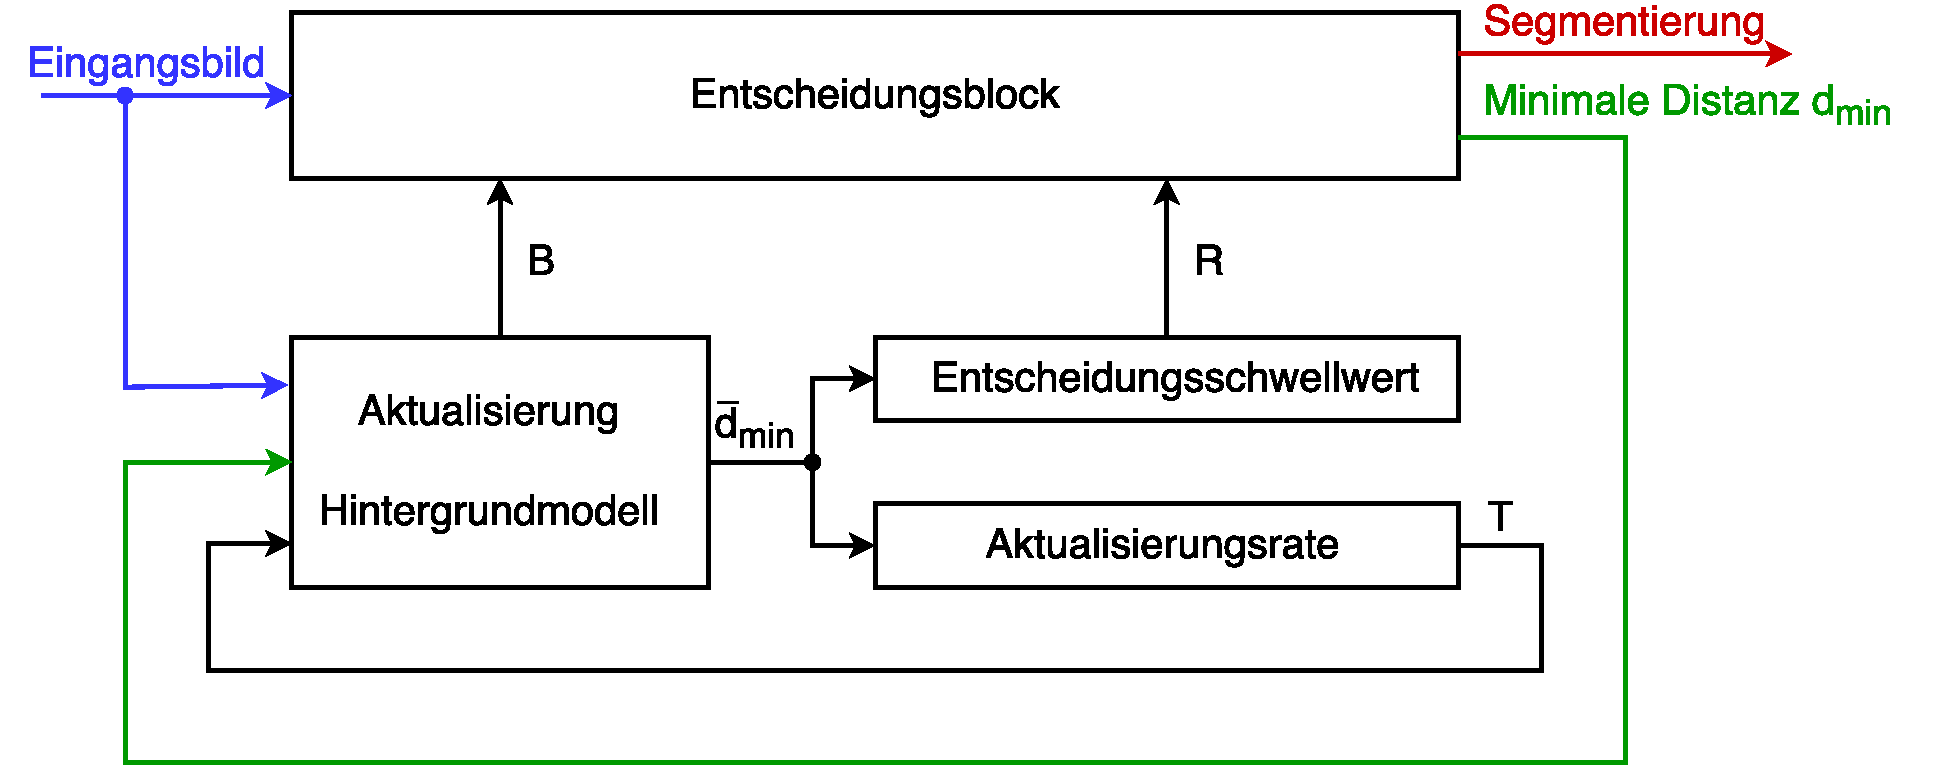
\includegraphics[width=\linewidth]{./Bilder/PDF/PBAS_Blockdiagramm.pdf}
	\end{figure}
	\begin{center}
		Blockschaltbild der Gesamtschaltung
	\end{center}
\end{frame}

\begin{frame}{Hintergrundmodelle}
	\begin{figure}
		\centering
		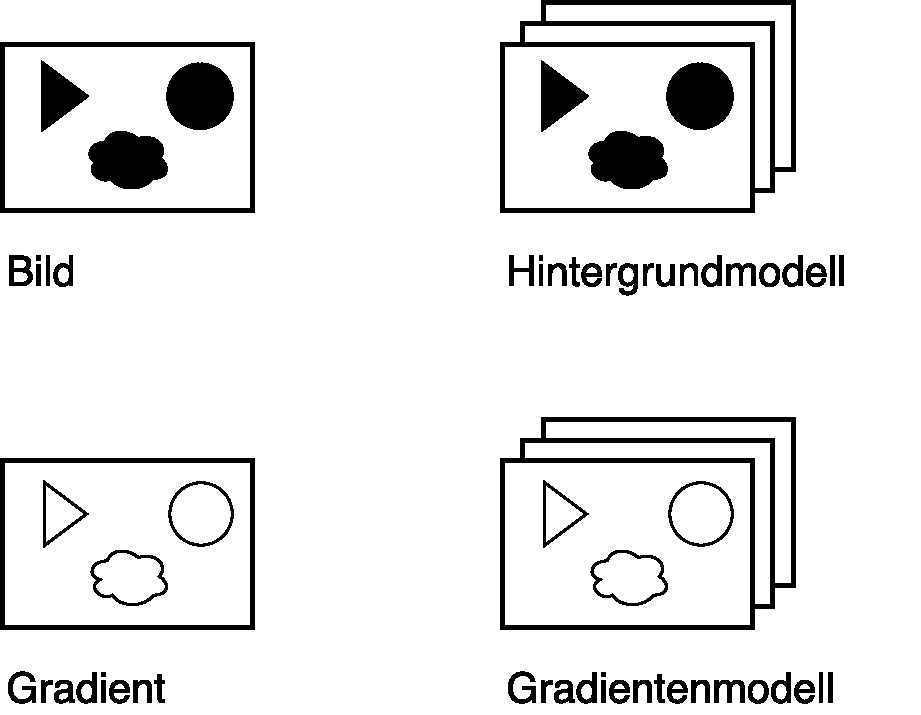
\includegraphics[width=.8\linewidth]{./Bilder/PDF/arrays.pdf}
	\end{figure}	
\end{frame}

\begin{frame}{Entscheidungsblock I}
	\begin{figure}
		\centering
		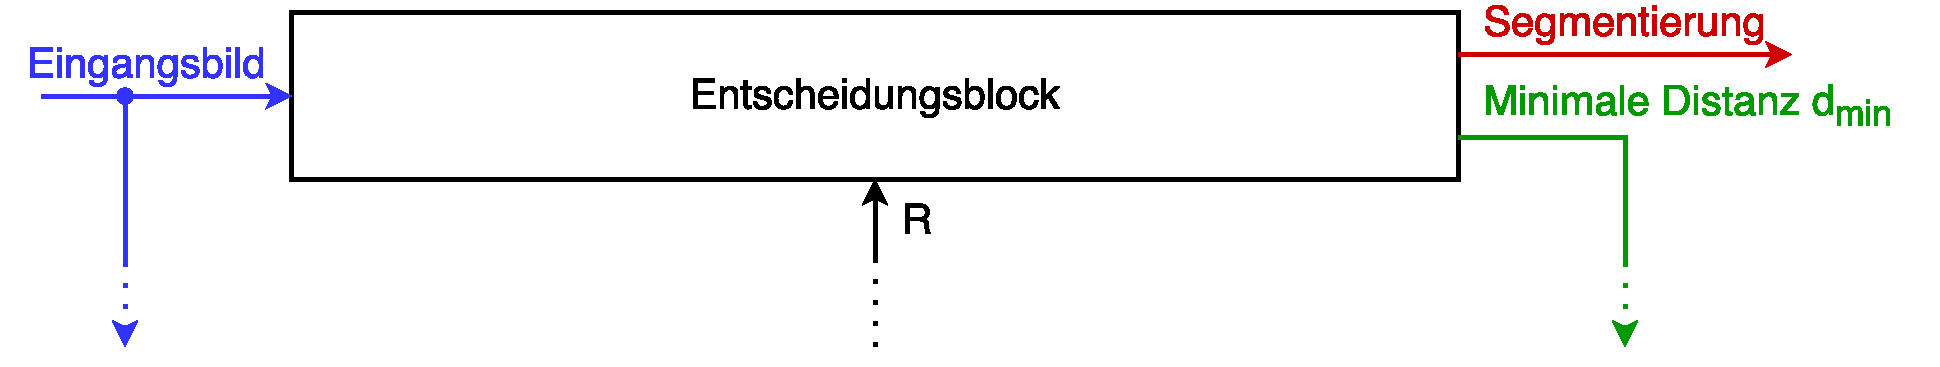
\includegraphics[width=\linewidth]{./Bilder/PDF/decision_block.pdf}
	\end{figure}

	\begin{center}
		\small
		$ Distanz = | Bild - Hintergrundmodell | + | Gradient - Gradientenmodell | $
	\end{center}
	
	\vspace{2em}
	
	$ F(x) = \left\{\begin{array}{ll} 1, & \#\left\{ Distanz < R \right\} < \#_{min} \\
				0, & sonst\end{array}\right. $
\end{frame}

\begin{frame}{Entscheidungsblock II}
	\begin{figure}
		\captionsetup[subfigure]{labelformat=empty}
		\begin{subfigure}{.3\linewidth}
			\centering
			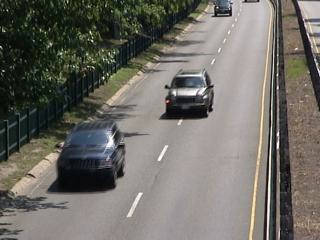
\includegraphics[width=\linewidth]{./Bilder/decision_bilder/orig}
			\caption{Original}
		\end{subfigure}
		\hspace{5mm}
		\begin{subfigure}{.3\linewidth}
			\centering
			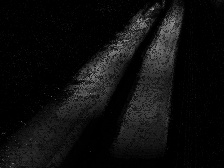
\includegraphics[width=\linewidth]{./Bilder/decision_bilder/distance}
			\caption{Distanz}
		\end{subfigure}
	
		\vspace{5mm}
		\begin{subfigure}{.3\linewidth}
			\centering
			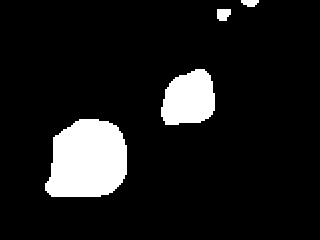
\includegraphics[width=\linewidth]{./Bilder/decision_bilder/foreground}
			\caption{Vordergrund}
		\end{subfigure}
	\end{figure}
\end{frame}

\begin{frame}{Aktualisierung Hintergrundmodelle I}
	\begin{figure}
		\centering
		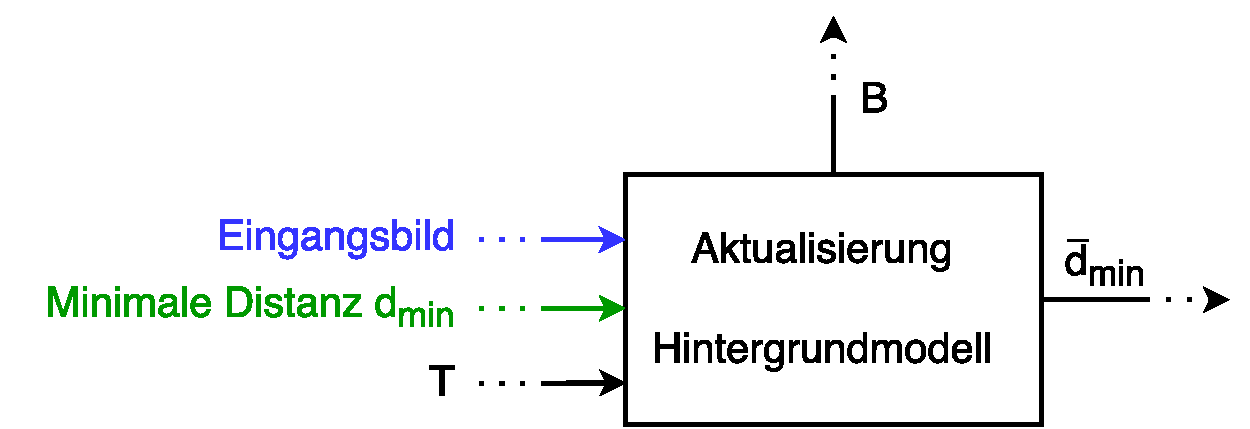
\includegraphics[width=\linewidth]{./Bilder/PDF/background_update}
	\end{figure}
	\begin{itemize}
		\item Aktualisiert \textbf{Hintergrund-} und \textbf{Gradientenmodell}
		\item Nur Hintergrundbereiche und zuf"allige Ebene
	\end{itemize}
\end{frame}

\begin{frame}{Aktualisierung Hintergrundmodelle II}
	\begin{figure}
		\captionsetup[subfigure]{labelformat=empty}
		\begin{subfigure}{.3\linewidth}
			\centering
			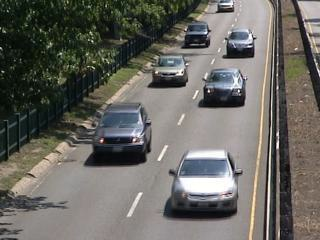
\includegraphics[width=\linewidth]{./Bilder/backup_bilder/orig0823}
			\caption{Original}
		\end{subfigure}
		\begin{subfigure}{.3\linewidth}
			\centering
			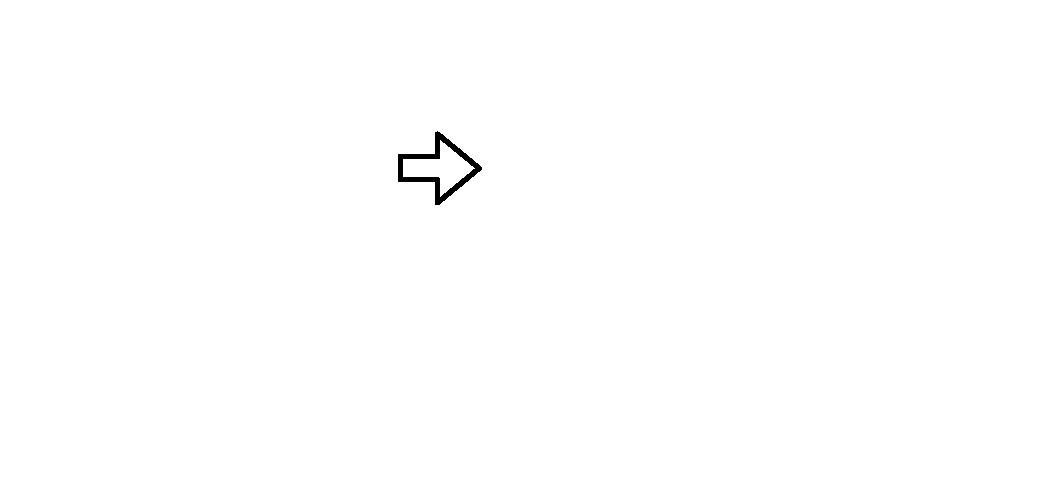
\includegraphics[width=1cm]{./Bilder/backup_bilder/pfeil.pdf}
		\end{subfigure}
		\begin{subfigure}{.3\linewidth}
			\centering
			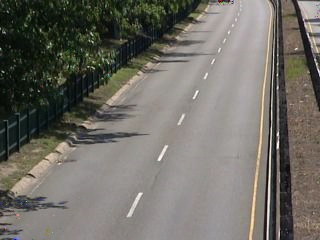
\includegraphics[width=\linewidth]{./Bilder/backup_bilder/hintergrundmodell0823}
			\caption{Hintergrundmodell}
		\end{subfigure}
	
		\vspace{5mm}
		\begin{subfigure}{.3\linewidth}
			\centering
			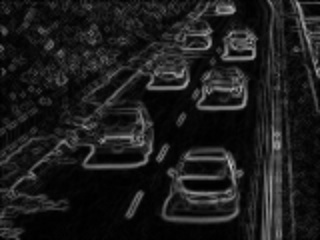
\includegraphics[width=\linewidth]{./Bilder/backup_bilder/gradient0823}
			\caption{Gradient}
		\end{subfigure}
		\begin{subfigure}{.3\linewidth}
			\centering
			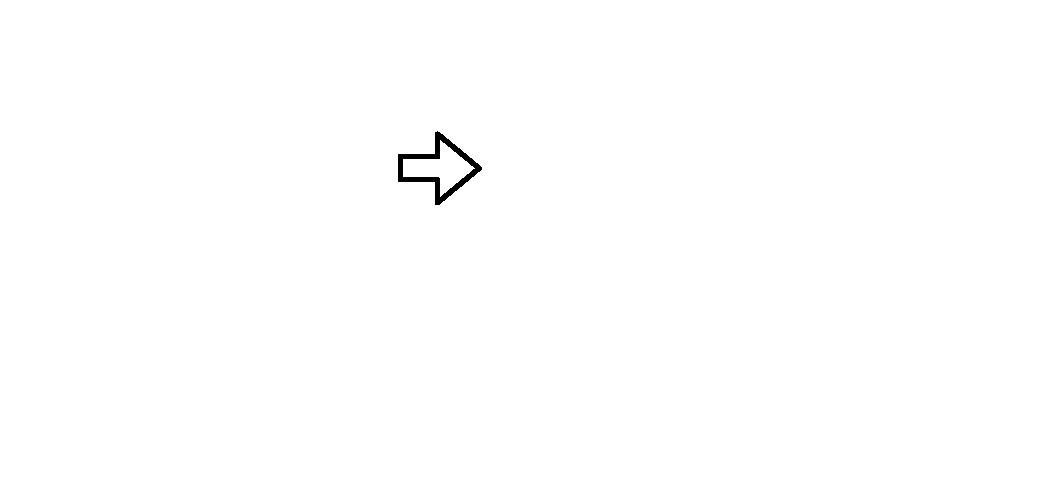
\includegraphics[width=1cm]{./Bilder/backup_bilder/pfeil.pdf}
		\end{subfigure}
		\begin{subfigure}{.3\linewidth}
			\centering
			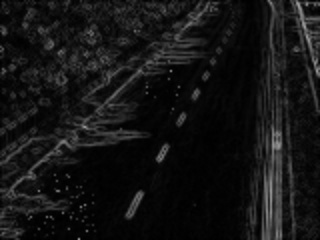
\includegraphics[width=\linewidth]{./Bilder/backup_bilder/gradientenmodell0823}
			\caption{Gradientenmodell}
		\end{subfigure}
	\end{figure}
\end{frame}

\begin{frame}{Aktualisierung Schwellwerte I}
	\begin{figure}
		\centering
		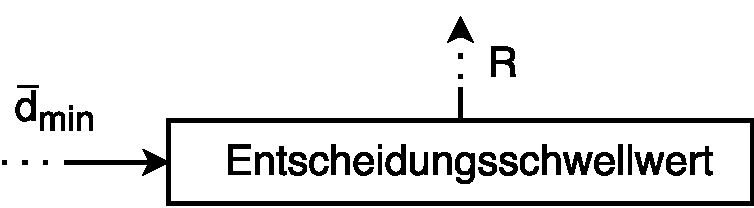
\includegraphics[width=.8\linewidth]{./Bilder/threshold_update/threshold_update}
	\end{figure}
	\vspace{2em}
	\begin{center}
		\Large
		$ R = \left\{\begin{array}{ll} R(1-R_{inc/dec}), & R < \overline{d}_{min}R_{scale} \\
		R(1+R_{inc/dec}), & sonst\end{array}\right.  $
	\end{center}
	
\end{frame}

\begin{frame}{Aktualisierung Schwellwerte II}
	\begin{figure}
		\captionsetup[subfigure]{labelformat=empty}
		\begin{subfigure}{.4\linewidth}
			\flushleft
			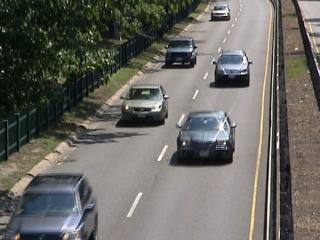
\includegraphics[width=\linewidth]{./Bilder/threshold_update/orig0850}
			\caption{Original}
		\end{subfigure}
		\hspace{10mm}
		\begin{subfigure}{.4\linewidth}
			\centering
			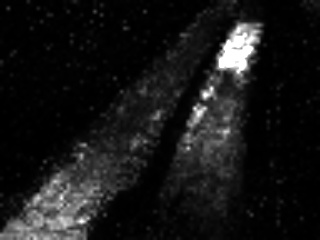
\includegraphics[width=\linewidth]{./Bilder/threshold_update/R_arr0850}
			\caption{Schwellwert}
		\end{subfigure}
	\end{figure}
\end{frame}

\begin{frame}{Aktualisierungsrate I}
	\begin{figure}
		\centering
		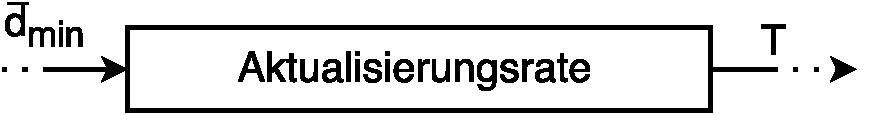
\includegraphics[width=.8\linewidth]{./Bilder/update_bilder/updaterate_update}
	\end{figure}
	\vspace{2em}
	\begin{center}
		\Large
		$ T = 	\left\{\begin{array}{ll} T + \frac{T_{inc}}{\overline{d}_{min}}, & F = 1 \\
				& \\
				T + \frac{T_{dec}}{\overline{d}_{min}}, & F = 0\end{array}\right.  $
	\end{center}
\end{frame}

\begin{frame}{Aktualisierungsrate II}
	\begin{figure}
		\captionsetup[subfigure]{labelformat=empty}
		\begin{subfigure}{.4\linewidth}
			\centering
			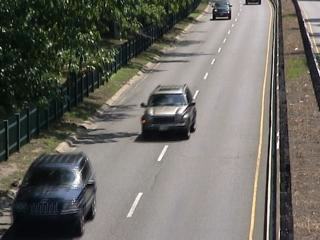
\includegraphics[width=\linewidth]{./Bilder/update_bilder/orig1198}
			\caption{Original}
		\end{subfigure}
		\hspace{10mm}
		\begin{subfigure}{.4\linewidth}
			\centering
			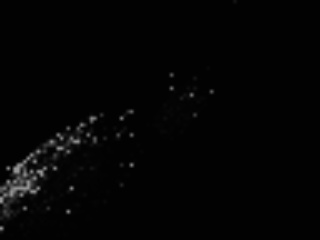
\includegraphics[width=\linewidth]{./Bilder/update_bilder/updatearr1198}
			\caption{Aktualisiuerungsrate}
		\end{subfigure}
	\end{figure}
	\vspace{1em}
	\begin{center}
		\Large
		$ Wahrscheinlichkeit = 1/Aktualisierungsrate $
	\end{center}
\end{frame}

\begin{frame}{Multiprocessing}
	\begin{figure}
		\centering
		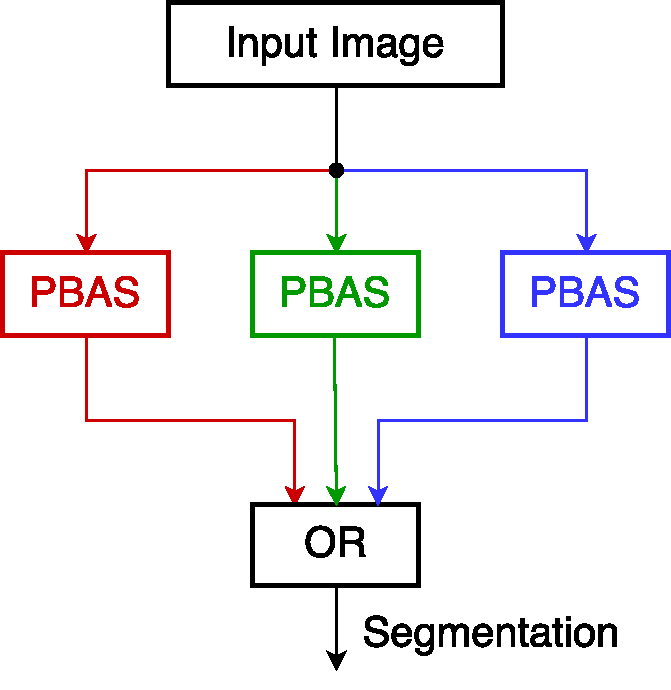
\includegraphics[width=.6\linewidth]{./Bilder/PDF/3channel_blockdiagramm}
	\end{figure}
\end{frame}

\end{document}
